\documentclass[aspectratio=169]{beamer}

\usepackage{tikz}
\usetikzlibrary{shapes, backgrounds, arrows, positioning}
\usepackage{pgfplots}
\usepackage{listings}
\usepackage[utf8,latin1]{inputenc}
\usepackage[style = apa, backend = biber, natbib = true]{biblatex}
\addbibresource{../../literature/lit.bib}

\makeatletter \def\newblock{\beamer@newblock} \makeatother  

\beamertemplatenavigationsymbolsempty
\setbeamertemplate{itemize items}[circle]
\setbeamertemplate{section in toc}[circle]
\mode<beamer>{\setbeamercolor{math text displayed}{fg=iwmgray}}
\setbeamercolor{block body}{bg=iwmorange!50!white}
\setbeamercolor{block title}{fg=white, bg=iwmorange}

% Definitions for biblatex
\setbeamercolor{bibliography entry note}{fg=iwmgray}
\setbeamercolor{bibliography entry author}{fg=iwmgray}
\setbeamertemplate{bibliography item}{}

\definecolor{iwmorange}{RGB}{255,105,0}
\definecolor{iwmgray}{RGB}{67,79,79}
\setbeamercolor{title}{fg=iwmorange}
\setbeamercolor{frametitle}{fg=iwmorange}
\setbeamercolor{structure}{fg=iwmorange}
\setbeamercolor{normal text}{fg=iwmgray}
\setbeamercolor{author}{fg=iwmgray}
\setbeamercolor{date}{fg=iwmgray}

\title{Simple linear regression}
\author{Nora Wickelmaier}
\date{October 24, 2022}
%\date{Last modified: \today}

\newcommand{\vect}[1]{\mathbf{#1}}
\newcommand{\mat}[1]{\mathbf{#1}}
\newcommand{\gvect}[1]{\boldsymbol{#1}}
\newcommand{\gmat}[1]{\boldsymbol{#1}}

\lstset{language=R,%
  %backgroundcolor=\color{iwmgray!80!white},
  basicstyle=\ttfamily\color{iwmorange},
  upquote=true,
  frame=single,
  commentstyle=\slshape\color{black},
  keywordstyle=\bfseries\color{white},
  identifierstyle=\color{white},
  stringstyle=\color{green!85!black},
  numbers=none,%left,numberstyle=\tiny,
  basewidth={.5em, .4em},
  showstringspaces=false,
  emphstyle=\color{red!50!white}}

\lstdefinestyle{plain}{language=R,
  frame=none,
  basicstyle=\ttfamily\color{iwmorange},
  commentstyle=\slshape\color{iwmgray},
  keywordstyle=\bfseries\color{iwmgray},
  identifierstyle=\color{iwmgray},
  stringstyle=\color{iwmgray},
  numbers=none,
  basewidth={.5em, .4em},
  showstringspaces=false}

\pgfmathdeclarefunction{gauss}{2}{%
  \pgfmathparse{1/(#2*sqrt(2*pi))*exp(-((x-#1)^2)/(2*#2^2))}%
}

\AtBeginSection[]{
  \frame{
    \tableofcontents[sectionstyle=show/hide, subsectionstyle=show/show/hide]}}

\setbeamertemplate{headline}{
 \begin{beamercolorbox}{section in head}
   \vskip5pt\insertsectionnavigationhorizontal{\paperwidth}{}{}\vskip2pt
 \end{beamercolorbox}
}

\setbeamertemplate{footline}{\vskip-2pt\hfill\insertframenumber$\;$\vskip2pt}

\begin{document}

\begin{frame}{}
\thispagestyle{empty}
\titlepage
\end{frame}

\begin{frame}{Outline}
\tableofcontents
\end{frame}


\begin{frame}{What is regression?}
  \pause
  Set of statistical processes for estimating the relationships between a
  dependent variable (often called the `outcome variable') and one or more
  independent variables (often called `predictors', `covariates', or
  `features')
  \flushright{\tiny{\url{https://en.wikipedia.org/wiki/Regression_analysis}}}
  \pause
\vfill
  \begin{itemize}
    \item Predict an outcome variable
    \item Compare predictions for different groups
    \item ``Find the line that most closely fits the data''
    \item Continuous outcome $Y$
  \end{itemize}
\end{frame}

\section{Basic concepts}

\begin{frame}{Simple linear regression}
  \begin{itemize}
    \item For the pairs
      \[
        (x_1, y_1), \ldots, (x_n, y_n),
      \]\\[2ex]
    we get the stochastical model
      \begin{align*}
        y_i & = \beta_0 + \beta_1 \cdot x_i + \varepsilon_i\\
        \varepsilon_i & \sim N(0, \sigma^2)~\text{i.i.d.}
      \end{align*}
for all $i = 1, \dots, n$
  \end{itemize}
\end{frame}

\begin{frame}{Simple linear regression}
  \begin{itemize}
    \item From the properties of the error variables, we conclude
\[
  E(y_i) = E(\beta_0 + \beta_1 \cdot x_i + \varepsilon_i) =
  \beta_0 + \beta_1 \cdot x_i = \bar{y}
\]
and
\[
  Var(y_i) = Var(\beta_0 + \beta_1 \cdot x_i + \varepsilon_i) = \sigma^2
\]
\item For a given $x_i$, the stochastical independence of $\varepsilon_i$
  transfers to $y_i$\\[2ex]
  \end{itemize}
\end{frame}

\begin{frame}{Simple linear regression}
\begin{columns}[c]
\begin{column}{6cm}
  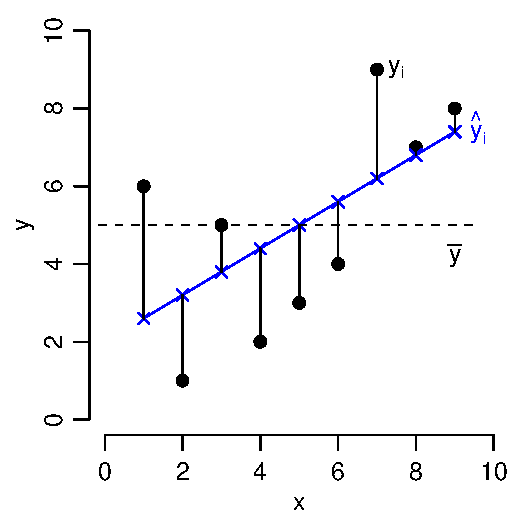
\includegraphics[scale=.7]{../figures/obs_pred}
\end{column}
%
\begin{column}{5cm}
{\small
\[
  s_y^2 = s_{\hat y}^2 + s_e^2
\]
\[
  \frac{1}{n} \sum_{i=1}^n (y_i - \bar{y})^2 =
\]
\[
  \frac{1}{n} \sum_{i=1}^n (\hat{y_i} - \bar{y})^2 +
  \frac{1}{n} \sum_{i=1}^n (y_i - \hat{y_i})^2
\]
}
\end{column}
\end{columns}
\vfill
\end{frame}

\begin{frame}{}
  \begin{block}{Exercise}
    \begin{itemize}
      \item Simulate a data set based on a simple regression model with
        \begin{align*}
          \beta_0 & = 0.2\\
          \beta_1 & = 0.3\\
          \sigma & = 0.5\\
          x & \in [1, 20]~\text{in steps of 1}
        \end{align*}
        \vspace{-.5cm}
      \item What functions in $R$ do we need?
    \end{itemize}
  \end{block}
\end{frame}

{\setbeamercolor{background canvas}{bg=iwmgray!80!white}

\begin{frame}[fragile]{Simulate data set}
\begin{lstlisting}
x <- 1:20
n <- length(x)
a <- 0.2
b <- 0.3
sigma <- 0.5
y <- 0.2 + 0.3*x + rnorm(n, sd=sigma)

dat <- data.frame(x, y)

# clean up workspace
rm(x, y)

# plot data
plot(y ~ x, dat)
\end{lstlisting}
  \nocite{GelmanHill2020}
\end{frame}

\begin{frame}[fragile]{Fit regression model}
\begin{lstlisting}
lm1 <- lm(y ~ x, dat)
summary(lm1)

mean(resid(lm1))
sd(resid(lm1))
hist(resid(lm1), breaks=15)

# plot data
plot(y ~ x, dat)
abline(lm1)
\end{lstlisting}
\end{frame}

\begin{frame}[fragile]{Re-cover parameters}
\begin{lstlisting}
pars <- replicate(2000, {
  ysim <- 0.2 + 0.3*x + rnorm(n, sd=sigma)
  lm1 <- lm(ysim ~ x, dat)
  c(coef(lm1), sigma(lm1))
})

rowMeans(pars)
# standard errors
apply(pars, 1, sd)

hist(pars[1, ])
hist(pars[2, ])
hist(pars[3, ])
\end{lstlisting}
\end{frame}

}

\begin{frame}{Sample distribution}
  \begin{center}
  \begin{tikzpicture}
\begin{axis}[every axis plot post/.append style={
  mark=none, domain=-4:4, samples=50, smooth},
    % All plots: from -2:2, 50 samples, smooth, no marks
  axis x line*=bottom, % no box around the plot, only x and y axis
  axis y line*=left,   % the * suppresses the arrow tips
  enlargelimits=upper] % extend the axes a bit to the right and top
\addplot[color=iwmorange, fill=iwmorange!50] {gauss(0, 1)};
%\addplot[color=iwmgray, fill=iwmgray!50, opacity=.5] {gauss(3, 1)};
\draw (axis cs: 0, 0) -- (axis cs: 0, .4);
  \draw[dashed] (axis cs: 0, .241) -- (axis cs: 1, .241);
  \draw[dashed] (axis cs: 1, 0) -- (axis cs: 1, .241);
\node[color=iwmorange] at (axis cs: 0, .42) {$\theta$};
  \node[color=iwmgray]   at (axis cs: 1.4, .241) {$se$};
\end{axis}
\end{tikzpicture}
  \end{center}
\end{frame}

\begin{frame}{}
  \begin{block}{Exercise}
    \begin{itemize}
      \item Simulate data with the parameters from slide~8
      \item Do not assume that we have one subject per value for $x$, but
        more than one subject
      \item Simulate data for $n=40$ and $n=100$\\
        Hint: Use \texttt{sample(x, n, replace=TRUE)}
      \item Re-cover your parameters as done on slide~11
      \item What happens to your standard errors?
    \end{itemize}
  \end{block}
\end{frame}

\section{Assumptions}

\begin{frame}{Assumptions}
  \begin{columns}
    \column{.6\textwidth}
    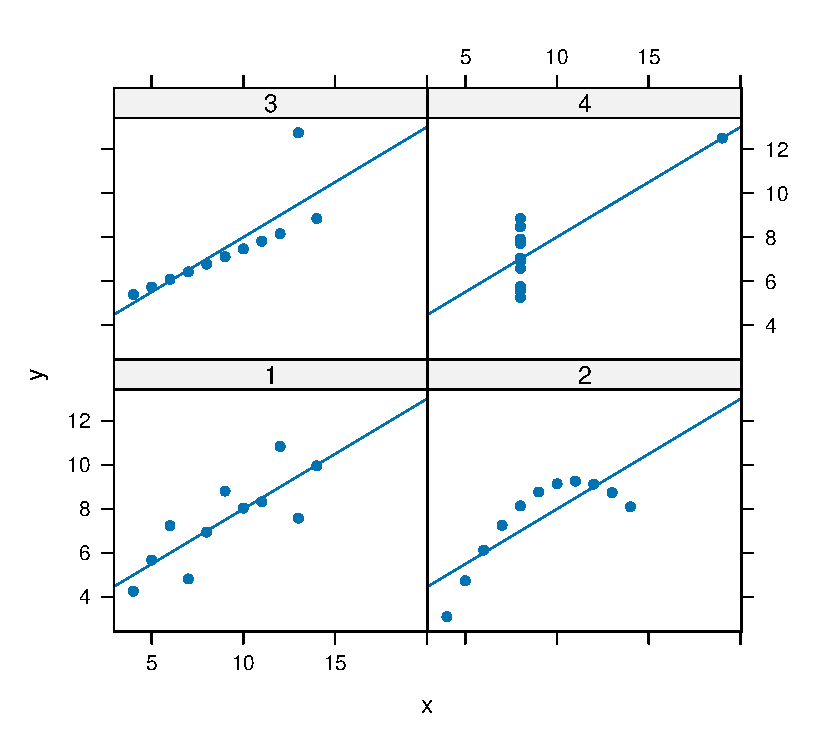
\includegraphics[scale=.61]{../figures/anscombe} 
    \column{.4\textwidth}
  \begin{itemize}
    \item Four data sets by \citet{Anscombe1973} with the same traditional
      statistical properties (mean, variance, correlation, regression line,
      etc.)
    \item Available in R with \texttt{data(anscombe)}
  \end{itemize}
  \end{columns}
\end{frame}

{\setbeamercolor{background canvas}{bg=iwmgray!80!white}

\begin{frame}[fragile]{Assumptions}
\begin{lstlisting}
data(anscombe)

lm1 <- lm(y1 ~ x1, anscombe)
lm2 <- lm(y2 ~ x2, anscombe)
lm3 <- lm(y3 ~ x3, anscombe)
lm4 <- lm(y4 ~ x4, anscombe)

rbind(coef(lm1), coef(lm2), coef(lm3), coef(lm4))

par(mfrow=c(2,2))
plot(lm1)
plot(lm2)
plot(lm3)
plot(lm4)
\end{lstlisting}
\end{frame}

}

\begin{frame}{Extending simple linear regression}
  \begin{tabular}{ll}
    Additional predictors &
      $y = \beta_0 + \beta_1 x_1 + \beta_2 x_2 + \dots +
      \varepsilon$\\
      & \\
    Nonlinear models &
      $\log y = \beta_0 + \beta_1 \log x + \varepsilon$\\
      & \\
    Nonadditive models &
      $y = \beta_0 + \beta_1 x_1 + \beta_2 x_2 + \beta_3
      x_1 x_2 + \varepsilon$\\
      & \\
    Generalized linear models &
      $g(E(y)) = \beta_0 + \beta_1 x$\\
      & \\
    Mixed-effects models &
      $y = \beta_0 + \beta_1 x_1 + \beta_2 time + 
      \upsilon_0 + \upsilon_1 time + \varepsilon$\\
      \dots & \\
  \end{tabular}
\end{frame}

\appendix

%\begin{frame}[allowframebreaks]{References}
\begin{frame}{References}
  %\renewcommand{\bibfont}{\footnotesize}
  \printbibliography
  \vfill
\end{frame}

\end{document}

